\documentclass[twocolumn,english]{IEEEtran}
\usepackage[T1]{fontenc}
\usepackage{babel}
\usepackage{amsthm}
\usepackage{amsmath}
\usepackage{graphicx}
\usepackage[unicode=true,
 bookmarks=true,bookmarksnumbered=true,bookmarksopen=true,bookmarksopenlevel=1,
 breaklinks=false,pdfborder={0 0 0},backref=false,colorlinks=false]
 {hyperref}
\usepackage{bm}
\usepackage{amsmath}
\usepackage{amssymb}
\usepackage{natbib}
\usepackage{siunitx}



\hypersetup{
 pdftitle=  {Lab 2: The Cathode Ray Tube},
 pdfauthor= {Zack Garza},
 pdfpagelayout=OneColumn, pdfnewwindow=true, pdfstartview=XYZ, plainpages=false}

\makeatletter


%%%%%%%%%%%%%%%%%%%%%%%%%%%%%% Textclass specific LaTeX commands.
 % protect \markboth against an old bug reintroduced in babel >= 3.8g
 \let\oldforeign@language\foreign@language
 \DeclareRobustCommand{\foreign@language}[1]{%
   \lowercase{\oldforeign@language{#1}}}
\theoremstyle{plain}
\newtheorem{thm}{\protect\theoremname}
\theoremstyle{plain}
\newtheorem{lem}[thm]{\protect\lemmaname}

%%%%%%%%%%%%%%%%%%%%%%%%%%%%%% User specified LaTeX commands.
% for subfigures/subtables
\ifCLASSOPTIONcompsoc
\usepackage[caption=false,font=normalsize,labelfont=sf,textfont=sf]{subfig}
\else
\usepackage[caption=false,font=footnotesize]{subfig}
\fi

\makeatother
\providecommand{\lemmaname}{Lemma}
\providecommand{\theoremname}{Theorem}
\sisetup{detect-weight=true, detect-family=true}

\begin{document}

\title{Lab 2: The Cathode Ray Tube}


\author{Zack Garza}


\IEEEspecialpapernotice
{Physics 215L \\
Effective Date of Report: February 25, 2014}


\markboth{Lab 2: The Cathode Ray Tube}{Zack Garza}
\maketitle
\begin{abstract}
The motivation for this experiment was to determine the deflection of the electron beam in a CRT tube as a function of applied voltage.
This information was used, in conjunction with derived equations, to find a ratio of $l/d$ in its deflection plates.
The theoretical value of $l/d$ was calculated to be \num{16.2}, while the experimental value was found to be \num{13.5}, which resulted in a percent error of \num{-16}\%.
\end{abstract}
\tableofcontents

\section{Introduction}



\IEEEPARstart{T}{he} cathode ray tube is the central component
of a number of familiar devices including the television set, the
personal computer and the oscilloscope.
In this experiment, you will
explore the characteristics of a CRT using the Demonstration Unit
$\#24-3010$.
This will result in the verification of the effective ratio
of length to spacing $(l/d)$ of the deflecting plates and to an understanding
of how the anodes focus the electron beam.
The concepts of electric field and electric potential will be reinforced and the information
gained will serve as valuable preparation for Experiment 7.

\section{Theory}
Referring to the accompanying schematic of the CRT and using the information provided by your instructor, derive an equation for the vertical deflection $y$ of the electron beam in terms of $L$, $l$, $d$, $V_1$, \& $V_2$.
All of the important quantities you will use are listed below:

\noindent
\begin{align*}
&y = \text{Beam deflection at the screen}\\
&q = \text{Electron Charge}\\
&E = \text{Electric field strength between plates (uniform)}\\
&F = \text{deflecting force (on q)} =qE\\
\end{align*}
\hrulefill \\

Given the above information, the equation for the total deflection is derived in Appendix~\ref{deriv} and is equal to
\begin{equation}\label{ydeflection}
  \Delta y_T = \Delta V_2 (\frac{l}{d})(\frac{l+2L}{4\Delta V_1}).
\end{equation}
The ratio of $l/d$ in this equation will be compared to the theoretical ratio of \num{16.2}.
\section{Methodology}

\subsection{Operation of the CRT}
  \begin{enumerate}
  \item
    Turn off the CRT unit ($\#24-3010$), and the Power Supply ($\text{EUW-}17$).
    Set the intensity control to a minimum (full CCW).  Set the power control to a minimum (full CCW).
    Now turn on the CRT and the Power Supply.\vspace{2pt}

    \textbf{CAUTION!  THE DEFLECTING PLATE TERMINALS AND THE SECOND ANODE ARE AT \num{700} VOLTS ABOVE GROUND.
    DON'T TOUCH THESE LEADS!}\vspace{2pt}
  \item
    Adjust the intensity control until a spot is visible on the screen.
    The spot should be no more intense than necessary to see it conveniently.
    A high intensity can burn the phosphor coating on the inside of the screen.
    Carefully measure the position of the spot using the grid on the screen.
    This will be your reference position for future spot positions.\vspace{2pt}

  \item
    Deflect the beam at equal voltage intervals ($V_2$) with an appropriate value that will result in no less than ten data points covering a complete screen deflection. Measure the position of the spot at each value of $V_2$. Record $V_1$ and ordered pairs of $V_2$ and $y$ (to \SI{0.1}{\milli\metre}) in Table 1.\vspace{2pt}

  \item
    When you are finished, turn the intensity and power supply controls to a minimum and turn off all the instruments (CRT unit, power supply, and voltmeters).
  \end{enumerate}

\subsection{Calculations}
  \begin{enumerate}
  \item
    Graph $y$ (mm) vs $V_2$ (volts).
    You should see a linear plot for which a curve fit will yield the slope.
    The number of decimal places you keep in the slope depends on the standard deviation on the slope of your graph!
    Calculate the ratio of $l/d$ (calculated), and compare this with $l/d$ (measured).
    Copy and paste your graph into this report. Don't forget to show sample calculations.\vspace{2pt}

  \item
    Complete the attached worksheet titled "CRT Electron Focusing".\vspace{2pt}

  \item
    Calculate $V_x$, the horizontal speed of the electron beam and attach this calculation to your report.\vspace{2pt}
  \end{enumerate}


\section{Results}
  \centerline{\underline{$ \Delta V_1 = 644 V$}}

  \begin{centering}
   \begin{table}[!htbp]
    \caption{y vs $\Delta V_2$}
    \centering{}
    \begin{tabular*}{\linewidth}{@{\extracolsep{\fill}} |c|c|c|}
    \hline
    \textbf{Trial} & \textbf{$\Delta V_2$ (volts)} & \textbf{$y$ (mm)} \\ \hline
    1  & 3.048  & 1  \\ \hline
    2  & 3.732  & 2  \\ \hline
    3  & 4.40   & 3  \\ \hline
    4  & 4.96   & 4  \\ \hline
    5  & 5.70   & 5  \\ \hline
    6  & 6.49   & 6  \\ \hline
    7  & 7.07   & 7  \\ \hline
    8  & 7.70   & 8  \\ \hline
    9  & 8.46   & 9  \\ \hline
    10 & 9.06   & 10 \\ \hline
    11 & 9.90   & 11 \\ \hline
    12 & 10.51  & 12 \\ \hline
    13 & 11.19  & 13 \\ \hline
    14 & 11.98  & 14 \\ \hline
    15 & 12.64  & 15 \\ \hline
    \end{tabular*}
   \end{table}
  \end{centering}
  Table 1 indicates the total deflection of the CRT electron beam as voltage was varied, where the beam was initially calibrated to align with $y=0$ on the superimposed grid.
  The voltage across the the focusing plates was kept constant at \SI{644}{\volt}, while the voltage supplied to the deflecting plates was steadily increased.
  Data points were taken when the beam aligned with a grid line. \\
  \begin{figure}[htbp]
   \begin{centering}
   \begin{center}
   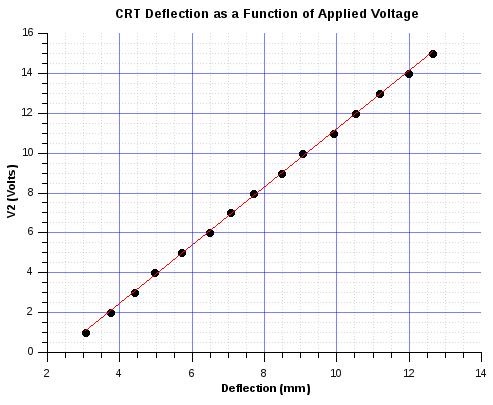
\includegraphics[keepaspectratio=true, width=\linewidth]{./CRTLab.png}
   % CRTLab.png: 493x405 pixel, 96dpi, 13.04x10.71 cm, bb=0 0 370 304
   \caption{Plot and Linear Regression of Table 1 Data}
   \end{center}
   \par\end{centering}
  \end{figure}

   \textbf{Linear Fit Data:}

  \begin{align*}
  \Delta y & =(1.458 \pm .008)\Delta V_2 - (3.359 \pm .07) \\
  R^2 & = 0.999590118089244 \\
  RMSE & = 0.0939586386136779
  \end{align*}
  Since the fit is linear, the equation is in the form $y=mx-b$.
  Inspection of equation~\ref{ydeflection} shows that if $y=\Delta y_T$ and $x=\Delta V_2$, then the slope must contain the remaining terms. That is,
  \begin{equation*}
  \frac{dy}{dV} = (\frac{l}{d})(\frac{l+2L}{4\Delta V_1})
  \Rightarrow (l/d) = \frac{dy}{dV}(\frac{4\Delta V_1}{l + 2L})
  \end{equation*}
  It is worth noting, however, that the slope is in units of (\si{\milli\metre\per\volt}), so with appropriate conversions, the linear fit yields that following ratio for $l/d$.
  \begin{align*}
    (l/d) &= \frac{dy}{dV}(\frac{4\Delta V_1}{l + 2L}) \\
	  &= (1.458\si{\milli\metre\per\volt})
	     \left(\frac{ (4)(644\si{\volt}) }{(38.0\si{\milli\metre})+2(120\si{\milli\metre})}\right)\\
	  &= (1.458\si{\milli\metre\per\volt})(\frac{2576\si{\volt}}{278\si{\milli\metre}})\\
	  &= 13.5
  \end{align*}
  Compared this to the accepted value calculated in the Theory section, the percent error is approximately $-16\%$.

  \hrulefill

  \textbf{Summary:}
  \begin{align*}
   &\text{Slope of Graph:} 	& 3.359 \pm .07 \,\si[per-mode=symbol]{\milli\metre\per\volt} \\
   &l/d \text{(graph):} 	& 13.5 \\
   &l/d \text{(manual):} 	& 16.2 \\
   & \%\text{error:} 		& -16\% \\
   &V_x 			& 1.51 \times 10^7 \si[per-mode=symbol]{\metre\per\second}\\
  \end{align*}
  \hrulefill



\section{Conclusions}

The results indicate that the derived expression and linear regression yielded a fairly accurate model of deflection as a function of applied voltage.
Error in this experiment arises from the fact that the plotted data does not accurately model what happens at small voltages.

The experimental setup was calibrated to a deflection \SI{0}{\milli\metre}, at which the applied voltage was equal to \SI{2.371}{\volt}.
However, the linear fit extrapolates a displacement of \SI{0}{\milli\metre} to a voltage of \SI{3.359}{\volt}, which is higher than the actual voltage by a factor of about \num{1.4}.

Reducing this error would involve taking more data points, potentially at lower voltages and negative deflections, to include these voltages in the data points.
Other sources of error may include electromagnetic interference, such as that of the Earth's own magnetic field which was observed to have a non-negligible effect on the CRT's deflection when its orientation was changed.


\appendices{}

\section{Derivation of Total Vertical Deflection}\label{deriv}

In order to calculate the total deflection in terms of the known quantities given in the theory section, the path of the electron can be examined in three stages: focusing, deflection, and the flight from the plates to the screen.
\begin{enumerate}
 \item \textbf{Focusing} \\
 Here, each electron is being accelerated in the $\hat{x}$ direction between two plates at a potential difference of $\Delta V_1$. From the Work-Kinetic Energy Theorem \cite{serway2013physics}, it can be stated that the initial potential will be equal to the final kinetic energy such that $q \Delta V_1 = \frac{1}{2}m{V_0}^2$. Thus the electron's speed entering part 2 can be expressed as

 \begin{equation} \label{eq:v0}
 {V_0}^2 = \frac{2q\Delta V_1}{m}
 \end{equation}

 \item \textbf{Deflection} \\
 In a similar manner, the electron is now accelerated in the $\mathbf{\hat{y}}$ direction due to the potential difference $\Delta V_2$ between the deflection plates. Neglecting the force of gravity, it follows a parabolic path that obeys kinematic equations. From Newton's Second Law, $F=ma$, where the net force is due to the electric field. Thus $ma = qE$ and

 \begin{equation}\label{eq:accel}
 a = \frac{qE}{m}
 \end{equation}

 The electric field $E$ is a function of the potential difference, where $\Delta V_2 = Ed \Rightarrow E = \Delta V_2/d.$ Substituting this into equation~\eqref{eq:accel} yields
 \begin{equation}\label{eq:accel2}
 a = \frac{q\Delta V_2}{md}
 \end{equation}

 Between the deflection plates, the electron will follow a parabolic path that obeys the kinematic equations. Integrating equation~\eqref{eq:accel2} twice (wrt time) yields
 \begin{equation}\label{eq:vy1}
  V_{y1} = (\frac{q\Delta V_2}{md})t_1
 \end{equation}
 \begin{equation}\label{eq:y1}
  \Delta y_1 = \frac{1}{2}(\frac{q\Delta V_2}{md}){t_1}^2
 \end{equation}
 Where $t_1$ is the time spent in the deflection chamber.


 Since the acceleration in the $\mathbf{\hat{x}}$ is 0, $\Delta x = V_0 t_1$ and $t_1=\Delta x/V_o.$ Since $\Delta x$ in the deflection plates is the known length $l$, this equation can be expressed as $t_1=l/V_o$. Substituting this into equation~\eqref{eq:y1} yields the following expression for the initial deflection.
 \begin{equation}\label{eq:y1final}
  \Delta y_1 = \frac{1}{2}(\frac{q\Delta V_2}{md}){(\frac{l}{V_0})}^2 =\frac{l^2 q\Delta V_2}{2md{V_0}^2}
 \end{equation}

 \item \textbf{Path to Screen} \\
 Neglecting gravity, the electron now has no net force acting upon it, and will continue on the trajectory at which it left the deflection plates. Because the distance from the plates to the screen is known to be $L$, $a_x=0$, and $V_x=V_0$, the kinematic equation of its motion in the $\mathbf{\hat{x}}$ is $\Delta x_2=V_0 t_2$ and thus
 \begin{equation} \label{eq:t2}
 t_2 = \frac{L}{V_0}
 \end{equation}

 Similarly, $a_y=0$, so $\Delta y_2 = (V_i \mathbf{\hat{y}})t$. To obtain $V_i \mathbf{\hat{y}}$, note that this will be equal to the particle's final velocity upon exiting the deflector. Since the time spent travelling through the deflector is known, from equation~\eqref{eq:vy1},
 \begin{align*}
  V_{y1} = (\frac{q\Delta V_2}{md})t_1 \Rightarrow V_{iy}= (\frac{q\Delta V_2}{md})(\frac{l}{V_0})
 \end{align*}
  Combining the above expression for $\Delta y_2$ and equation~\eqref{eq:t2} yields
  \begin{equation} \label{eq:y2final}
   \Delta y_2 = (\frac{q\Delta V_2}{md})(\frac{l}{V_0})(\frac{L}{V_0}) = \frac{l L q\Delta V_2}{md{V_0}^2}
  \end{equation}

  \item {\textbf{Total Deflection}}\\
  Finally, combining and simplifying equations~\eqref{eq:v0},~\eqref{eq:y1final}, and~\eqref{eq:y2final} yields the expression for the total deflection of the particle in terms of known quantities.

  \begin {align*}\label{eq:final}
   \Delta y_T & = \Delta y_1 + \Delta y_2 = \frac{l^2 q\Delta V_2}{2md{V_0}^2} + \frac{l L q\Delta V_2}{md{V_0}^2} \notag \\
   & = (\frac{q \Delta V_2 l^2 + 2lLq\Delta V_2}{2md})(\frac{m}{2q\Delta V_1}) \notag \\
   & = \frac{\Delta V_2 l^2 + 2lL\Delta V_2}{4d\Delta V_1}\notag \\
   & = \Delta V_2 (\frac{l}{d})(\frac{l+2L}{4\Delta V_1}) &&\blacksquare
  \end {align*}

\end{enumerate}

\section{Calculating the Electron's Horizontal Speed}\label{vx_calc}

 Considering equation~\ref{eq:v0}, and substituting known quantities for the supply voltage $\Delta V_1$, the electrons mass ($m_e =$ \SI{9.109e-31}{\kilo\gram}), and charge ($q_e=$ \SI{1.602e-19}{\coulomb}), the electron's speed (neglecting relativistic effects) is calculated as

 \begin{align*}
   {V_x} &= \sqrt{\frac{2q_e \Delta V_1}{m_e}} \\
   &=\sqrt{\frac{2(1.602 \times 10^{-19}\si{\coulomb})(644\si{\volt})}{9.109 \times 10^{-31}\si{\kilo\gram}}} \\
   &=1.51 \times 10^7 \si[per-mode=symbol]{\metre\per\second}
 \end{align*}



\bibliographystyle{plain}
\bibliography{physbib}

\end{document}